\documentclass{article}
\usepackage[slovak]{babel}
\usepackage[utf8]{inputenc}

\usepackage{indentfirst}
\usepackage{graphicx}

\begin{document}
    \begin{titlepage}
        \begin{center}
            \vspace{\stretch{0.382}}
            
            
\includegraphics[width=10cm]{FITlogo.png}\\[30mm]
            
            \LARGE
            Implementácia prekladača imperatívneho jazyka IFJ17 \\
            \large
            Dokumentácia k~projektu IFJ/IAL\\[55mm]
            
            \begin{tabular}{r l l}
                Tím: & 094 & \\
                Varianta: & II & \\
                Vedúci: & Tomáš Nereča (xnerec00) & 26\% \\
                Ďalší členovia: & Samuel Obuch (xobuch00) & 26\% \\
                    & Jiří Vozár (xvozar04) & 26\% \\
                    & Ján Farský (xfarsk00) & 22\% \\
                Implementované rozšírenia: & BASE, FUNEXP, IFTHEN &\\
            \end{tabular}
            
            \vspace{\stretch{0.618}}
        \end{center}
    \end{titlepage}

    \tableofcontents
    \newpage
    
    \section{Úvod}
        Dokumentácia popisuje implementáciu prekladača imperatívneho jazyka IFJ17. Prekladač načítava
        zdrojový kód jazyka IFJ17 zo~štandardného vstupu a ten pomocou lexikálnej, syntaktickej a sémantickej
        analýzy vyhodnotí a vygeneruje potrebné inštrukcie v~IFJcode17 pre interpret. V~prípade
        výskytu chyby pri analýze kódu IFJ17 prekladač vráti kód príslušnej chyby a chybovú hlášku na štandardný
        chybový výstup.
        
        Dokumentácia taktiež zahŕňa zhodnotenie práce v~tíme a približuje logiku a fungovanie
        jednotlivých častí prekladača. 
    
    \section{Implementácia}
    
        \subsection{Lexikálna analýza}
        Hlavná funkcia lexikálneho analyzátora je \texttt{getNextToken}. Je implementovaná v súbore \emph{scanner.c}.
        Jej argumenty sú ukazatele na štruktúru typu \emph{tToken} a \emph{FILE} a jej návratový typ je \emph{bool}. 

        Funkcia číta lexémy zo zadaného súboru(spravidla \emph{stdin}). Lexémy sú spracované pomocou konečného automatu. 
        Ak sa automat dostane do konečného stavu, funkcia vráti hodnotu \emph{true} a podľa spracovaných lexém nastaví
        token predaný v argumente. Ak nastane počas lexikálnej analýzy chyba, vráti funkcia hodnotu \emph{false} a 
        token nenastavuje. 

        Dátová štruktúra \emph{tToken} a jej podštruktúry sú definované v hlavičkovom súbore \emph{scanner.h}. 
        Platný token musí mať vždy definovaný typ, a ak to typ tokenu vyžaduje tak aj atribút 
        (napr. načítaný reťazec v prípade, že je token typu \emph{string}). 

        Funkcia \emph{getNextToken} sa taktiež stará o prevod veľkých písmen na malé a počítanie riadkov.
        Taktiež uľahčuje prácu syntaktickému analyzátoru, pretože rozlišuje medzi identifikátormi a kľučovými slovami.
        V poli reťazcov sú uložené všetky kľúčové slová a \emph{binárnym vyhľadávaním} vo funkcii \texttt{identifierTest} 
        sa testuje, či sa jedná o identifikátor alebo kľúčové slovo.

        Diagram konečného automatu nájdete v prílohe.

        \subsection{Syntaktická analýza}
            Prekladač využíva syntaxou riadený preklad, v ktorom kombinuje \emph{rekurzívny zostup} pre základné konštrukcie
            a príkazy jazyka s \emph{precedenčnou syntaktickou analýzou} pre výrazy.
            Vstupným bodom prekladača je funkcia \texttt{parse}, ktorá zavolá vyhodnotenie hlavného neterminálu \emph{program},
            ktorý po kontrole volá funkcie z neho vychádzajúcich ďalších neterminálov.
            Pokiaľ pravidlo očakáva výraz, je zavolaná funkcia \texttt{expression}, ktorá se postará o vyhodnotenie výrazu prevodom
            do postfixovej podoby.
            
            \subsubsection{Rekurzívny zostup}
                Pre každý neterminál je vytvorená funkcia, ktorá je volaná pre vyhodnotenie daného neterminálu.
                Funkcia potom vracia hodnotu \texttt{true}, pokiaľ bolo vyhodnotenie úspešné a hodnotu \texttt{false}, pokiaľ došlo k nejakej chybe. Niektoré funkcie z dôvodu zjednodušenia nereprezentujú pravidlá úplne presne, kedy se napríklad funkcia \texttt{statementList} nevolá rekurzívne, ale je riadená cyklom. Samotný zostup je rozdelený do 3 modulov pre oddelenie obecných neterminálov, neterminálov príkazov a neterminálov funkcií.
            
            \subsubsection{Precedenčná syntaktická analýza}
                Precedenčná syntaktická analýza je založená na precedenčnej tabuľke a prevode infixových výrazov
                na postfix, z ktorého sú následne generované zásobníkové inštrukcie IFJcode17. 

                Pri nájdení výrazu je zavolaná funkcia \texttt{expression}, ktorá ako argument dostane očakávaný
                výstupný typ tokenu. Na základe tohoto očakávaného tokenu kontrolujeme pri vytváraní \emph{postfixového 
                výrazu} pomocou funkcie \texttt{postfix} povolené dátové typy vo výraze. Na každý token je zavolaná 
                funkcia \texttt{getTerm}, ktorá v prípade ak sa vo výraze nachádza premenná alebo funkcia overí či 
                boli deklarované, funkcia vracia index tokenu z precedenčnej tabuľky a typ spracovaného tokenu. Ak 
                vyhodnotenie operandu alebo operácie vo funckii \texttt{postfix} prebehlo korektne je zavolaná funkcia 
                \texttt{generateInstruction} na vygenerovanie zásobníkovej inštrukcie pre daný token. Funkcia 
                \texttt{postfix} spracúva dalšie tokeny až pokým nenarazí na koniec výrazu. Ak preklad na \emph{postfix}
                prebehol úspešne funkcia \texttt{expression} vracia hodnotu \texttt{true}, v prípade chyby sa vypíše chybové
                hlásenie a funkcia vracia hodnotu \texttt{false}.
    
        \subsection{Tabuľka symbolov}
            Tabuľka symbolov je implementovaná ako hash tabuľka. Hashovacia funkcia bola zvolená \emph{djb2}\footnote{\texttt{http://www.cse.yorku.ca/\~{}oz/hash.html}}, pretože dávala dobré výsledky rozloženia pri experimentovaní s väčším množstvom záznamov.
            
            Veľkosť poľa pre ukazatele bola zvolená $128$ aby sa operácie modulo v hashovacej funkcii previedla na bitové maskovanie a pre bežný počet premenných vo funkcii je dostačujúci.
            
            Informácie o symbole sú následne ukladané v štruktúre, ktorá bola navrhnutá univerzálne pre informácie o premenných aj funkciách.
        
        \subsection{Vstavané funkcie}
            V prekladači sme implementovali aj štyri vstavané funkcie pre jazyk IFJ17.
            
            \subsubsection{Length}
            Vstupným parametrom funkcie je string a výstupným je číselná hodnota dĺžky vstupného stringu.
            
            \subsubsection{SubStr}
            Vstupné parametre funkcie sú string  a dva integery. Výstupom je podreťazec vstupného
            stringu, ktorého začiatok je určený prvým integerom a jeho dĺžka druhým. Ak je index dĺžky
            0 alebo indexujeme mimo medze stringu návratovou hodnotou je prázdny reťazec. Ak by časť 
            znakov podreťazca pripadala mimo medze základného stringu návratovou hodnotou je string
            obsahujúci iba znaky z~medzí vstupného stringu.
            
            \subsubsection{Asc}
            Vstupné parametre funkcie sú reťazec string a integer. Výstupnou hodnotou je ordinálna
            hodnota (ASCII) znaku v~stringu na pozícii zadanej integerom. Ak integer zasahuje mimo 
            medze stringu návratovou hodnotou je 0.
            
            \subsubsection{Chr}
            Vstupným parametrom je integer. Výstupom je znak, ktorého ASCII kód bol zadaný integerom.
            V~prípade integeru momo medzí 0-255 je chovanie funkcie nedefinované.
            
        \subsection{Generovanie kódu}
            Cieľový kód je generovaný priamo počas jediného priechodu vypisovaním príslušných inštrukcií vo funkcii
            príslušného pravidla.
            
            Premenné definované užívateľom sa ukladajú na dátový rámec, ktorý sa pre funkcie
            vytvorí vždy nový.
            Výrazy využívajú pre medzivýsledky zásobník, kam sa ukladajú aj vyhodnotené parametry a výsledky funkcií.
            
            Podmienky a cykly využívajú inštrukcie podmienených a nepodmienených skokov, ale funkcie se volajú inštrukciami \texttt{CALL}
            a \texttt{RETURN}.
        
    \section{Rozšírenia}
    Boli implementované celkom 3 rozšírenia
        \begin{itemize}
            \item \textbf{base}   - Lexikálny analyzátor dokáže prečítať celé číslo zadané v inej než
                                    desiatkovej sústave a následne ho previesť pomocou funkcie 
                                    \emph{strtol} s argumentom príslušnej číselnej sústavy do \emph{integeru}.
            \item \textbf{funexp} - Vďaka vhodnému návrhu nezávislého vyhodnocovania výrazov a predávaní parametrov funkcií
                                    cez zásobník ako výsledky rekurzívne volaných podvýrazov bolo toto rozšírenie implementované
                                    už v základnej verzii prekladača.
            \item \textbf{ifthen} - Podpora \emph{elseif} a možnosť vynechania \emph{else} obnášala iba ľahkú úpravu funkcie
                                    pre vyhodnocovanie podmienok prepísaním do cyklu a rozšírením generovánia inštrukcií
                                    pre skoky a náveštia.
        \end{itemize}
    
    \section{Testovanie}
    Na začiatku sme určili jedného člena, ktorý písal jednotkové testy pre lexikálny analyzátor.
    Jednotkové testy boli napísané v jazyku C...
    
    Neskôr sme napísali zopár vlastných regresných testov, tieto testy sme už písali v jazyku \emph{Python}, kde
    sme na vstup nášho prekladača posielali zdrojový kód IFJ17, jeho výstup v prípade ak nenastala chyba sme posielali
    do interpretu a výstup interpretu sme uložili do súboru. Na záver sme porovnali očakávaný výstup so získaným výstupom
    z interpretu alebo chybovým hlásením z prekladača. Ak sa výstupy zhodovali test prebehol úspešne ak nie test zlyhal.
    
    Keď sme sa dozvedeli o~verejnej databáze testov našich kolegov. Do ktorej sme prispeli aj vlastnými testami a využili ostatné testy na čo najrobustnejšie otestovanie funkčnosti nášho prekladača.
    
    \section{Práca v~tíme}
    Ako tím sme sa začali schádzať pomerne skoro po zaregistrovaní nášho zadania. Stretnutie sme mali 
    minimálne raz týždenne, kde sme prediskutovali aktuálny stav práve implementovaných častí 
    a ďalší postup či korekciu v~zdrojovom kóde. Prácu sme sa snažili rozdeľovať rovnomerne medzi 
    všetkých členov tímu čo sa nie vždy darilo. Po pridelení úlohy sme stanovili deadline, aby sme 
    mohli čo najskôr pokračovať na nasledujúcej časti projektu. Jednotlivé časti sme sa snažili 
    implementovať paralelne s~preberanou látkou na prednáškach aby sme korektne implementovali
    jednotlivé časti a vyhli sa zbytočným chybám.

        \subsection{Správa zdrojového kódu}
        Pre správu a zdielanie zdrojových súborov sme využili verzovací systém \emph{Git} a webovú službu GitHub pre vzdialené ukladanie, ktorú sme už 
        počas štúdia využili na verzovanie projektov v~iných predmetoch.
        
        Ako komunikačný kanál sme 
        prevažne využívali skupinovú konverzáciu na sociálnej sieti Facebook, ktorá nám všetkým 
        vyhovovala.
        
        Na sledovanie postupu pri plnení pridelených úloh a oznamovanie nájdených chýb 
        sme využívali online nástroj Trello, ktorý slúži ako online kanban pre sledovanie projektov. 
        
        Vďaka týmto informačným kanálom mohli mať všetci členovia tímu prístup k~najaktuálnejšej
        verzii projektu a reagovať na vzniknuté chyby efektívne.

        \subsection{Rozdelenie práce v tíme}

        \textbf{Tomáš Nereča} pracoval na lexikálnom analyzátore a v neskoršej fáze vývoja spolupracoval so \textbf{Samuelom Obuchom} na 
        precedenčnej syntaktickej analýze. Okrem toho sa podieľal na menších moduloch errors, stack a ifunc. 

        \textbf{Jiří Vozár} měl na starosti vedení implementace, návrh komunikace mezi moduly a implementaci syntaktické analýzy rekurzivním sestupem.

        Dôvod nerovnomerného rozdelenia bodov bolo nedostatočné splnenie pridelených častí jednému 
        z~členov tímu, čo viedlo k~potrebnému prepisu zdrojového kódu ostatnými členmi tímu.

    \section{Záver}
    S~projektom podobného rozsahu sa ešte nikto z~nás predtým nestretol, preto ho pokladáme za dobrú
    skúsenosť pre každého z~nás. Pri jeho riešení sme prakticky využili získané vedomosti z~predmetov 
    IFJ a IAL.
    
    Pre správne fungovanie tímu bola potrebná dobrá komunikácia, riadenie a pridelovanie úloh, ktoré pretvali počas celého
    priebehu projektu či už vďaka pravidelným stretnutiam alebo využitým nástrojom ale aj individuálne
    schopnosti jednotlivých členov. Výsledkom tejto práce je funkčný a z~nášho pohľadu vydarený 
    prekladač jazyka IFJ17.
    
    \newpage
    \section{Prílohy}
        \subsection{Diagram konečného automatu}
            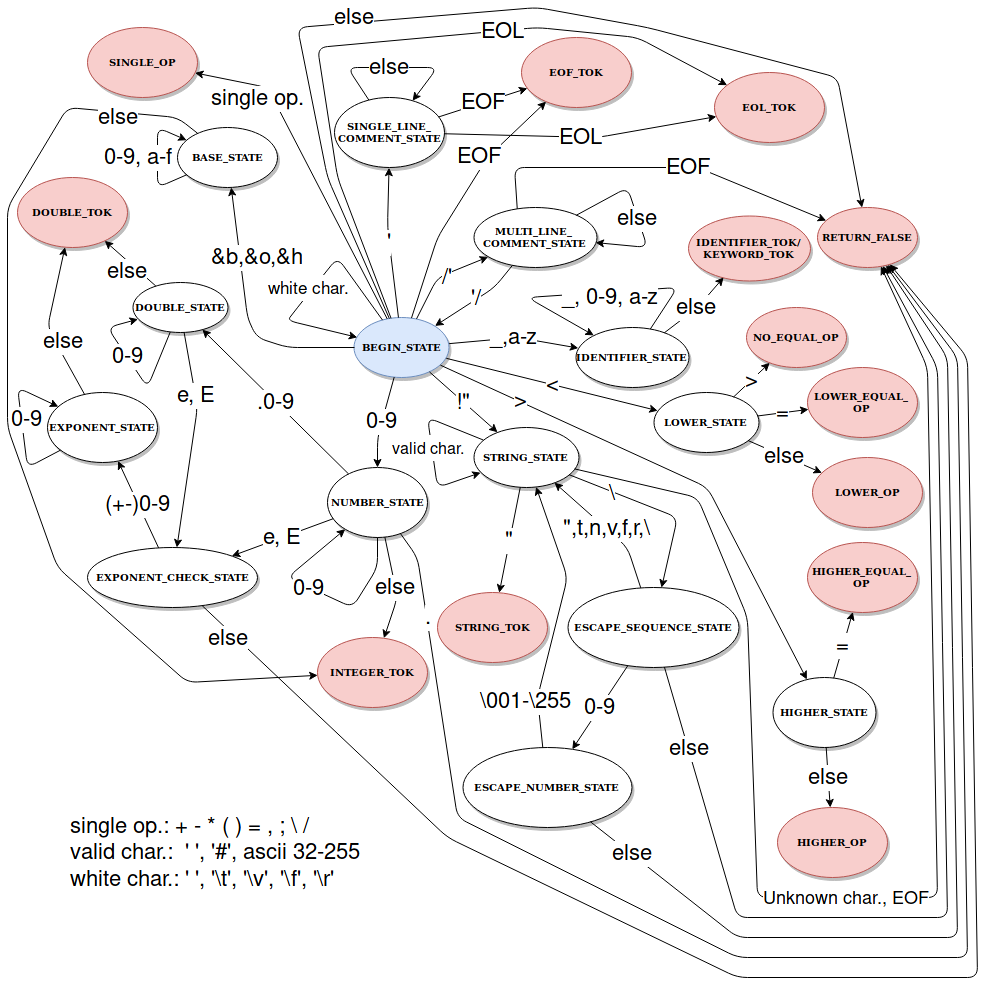
\includegraphics[trim=6cm 0 0 0, width=15cm]{finite_automata.png}
            \newpage
            
        \subsection{LL gramatika}
            \begin{enumerate}
                % NESAHAT - zhenodnotí čísla v tabulce LL gramatiky!
                \item \texttt{<program> -> declare function <functionDecl> eol <program>}
                \item \texttt{<program> -> function <functionDef> eol <program>}
                \item \texttt{<program> -> scope <statementList> end scope}
                
                \item \texttt{<functionDecl> -> <functionHeader>}
                \item \texttt{<functionDef> -> <functionHeader> eol <statementList> end function}
                
                \item \texttt{<functionHeader> -> identifier ( <functionParams> ) as type}
                
                \item \texttt{<functionParams> -> <functionParam> <nextFuncParam>}
                \item \texttt{<functionParams> -> epsilon}
                
                \item \texttt{<nextFuncParam> -> , <functionParam> <nextFuncParam>}
                \item \texttt{<nextFuncParam> -> epsilon}
                
                \item \texttt{<functionParam> -> identifier as type}
                
                \item \texttt{<statementList> -> <statement> eol <statementList>}
                \item \texttt{<statementList> -> epsilon}
                
                \item \texttt{<statement> -> dim <declaration>}
                \item \texttt{<statement> -> identifier = <expression>}
                \item \texttt{<statement> -> input identifier}
                \item \texttt{<statement> -> print <printArgs>}
                \item \texttt{<statement> -> if <expression> then eol <statementList> <else>}
                \item \texttt{<statement> -> do while <expression> eol <statementList> loop}
                \item \texttt{<statement> -> return identifier}
                
                \item \texttt{<declaration> -> identifier as type}
                \item \texttt{<declaration> -> identifier as type = <expression>}
                
                \item \texttt{<printArgs> -> <expression> ;}
                \item \texttt{<printArgs> -> <expression> ; <printArgs>}
                
                \item \texttt{<else> -> elseif <expression> then eol <else> end if}
                \item \texttt{<else> -> else eol <statementList> end if}
                \item \texttt{<else> -> end if}
                
                \item \texttt{<expression> ->} vyhodnocuje se precedenční syntaktickou analýzou
            \end{enumerate}
        \newpage
        
        \subsection{LL tabuľka}
        \newcommand{\tterm}[1]{\rotatebox[origin=c]{90}{\texttt{#1}}}
            \begin{tabular}{|r|*{10}{c|}}
                \hline
                & \tterm{declare} & \tterm{function} & \tterm{scope} & \tterm{identifier} & \tterm{dim} &
                \tterm{input} & \tterm{print} & \tterm{if} & \tterm{do} & \tterm{return} \\\hline \hline
                \texttt{<program>} & 1 & 2 & 3 &&&&&&& \\\hline
                \texttt{<functionDecl>} &&&& 4 &&&&&& \\\hline
                \texttt{<functionDef>} &&&& 5 &&&&&& \\\hline
                \texttt{<functionHeader>} &&&& 6 &&&&&& \\\hline
                \texttt{<functionParams>} &&&& 7, 8 &&&&&& \\\hline
                \texttt{<nextFuncParam>} &&&&&&&&&& \\\hline
                \texttt{<functionParam>} &&&& 11 &&&&&& \\\hline
                \texttt{<statementList>} &&&& 12 & 12 & 12 & 12 & 12 & 12 & 12 \\\hline
                \texttt{<statement>} &&&& 15 & 14 & 16 & 17 & 18 & 19 & 20 \\\hline
                \texttt{<declaration>} &&&& 21, 22&&&&&& \\\hline
                \texttt{<else>} &&&& 23, 24&&&&&& \\\hline
            \end{tabular}
            
            \begin{tabular}{|r|*{9}{c|}}
                \hline
                & \tterm{elseif} & \tterm{else} & \tterm{end} & \tterm{loop} & \tterm{eol} &
                \tterm{(} & \tterm{)} & \tterm{=} & \tterm{,} \\\hline \hline
                \texttt{<program>} &&&&&&&&& \\\hline
                \texttt{<functionDecl>} &&&&&&&&& \\\hline
                \texttt{<functionDef>} &&&&&&&&& \\\hline
                \texttt{<functionHeader>} &&&&&&&&& \\\hline
                \texttt{<functionParams>} &&&&&&& 8 && \\\hline
                \texttt{<nextFuncParam>} &&&&&&& 10 && 9 \\\hline
                \texttt{<statementList>} & 13 & 13 & 13 & 13 &&&&& \\\hline
                \texttt{<statement>} &&&&&&&&& \\\hline
                \texttt{<declaration>} &&&&&& 23, 24&&& \\\hline
                \texttt{<else>} & 25 & 26 & 27 &&&&&& \\\hline
            \end{tabular}
        \newpage

        \subsection{Precedenčná tabuľka}

        \begin{center}
        \begin{tabular}{|c|c|c|c|c|c|c|c|c|c|c|c|c|c|c|c|c|c|c|}
        \hline
                  & =(výraz) & $<>$ & $<$= & $>$= & $<$ & $>$ &  +  &  -  &  */  & \textbackslash &  (  &  )  & \$  \\ 
        \hline
        =(výraz)  &     $>$  &  $>$ &  $>$ &  $>$ & $>$ & $>$ & $<$ & $<$ &  $<$ & $<$            & $<$ & $>$ & $>$ \\ 
        \hline
          $<>$    &     $>$  &  $>$ &  $>$ &  $>$ & $>$ & $>$ & $<$ & $<$ &  $<$ & $<$            & $<$ & $>$ & $>$ \\
        \hline
          $<$=    &     $>$  &  $>$ &  $>$ &  $>$ & $>$ & $>$ & $<$ & $<$ &  $<$ & $<$            & $<$ & $>$ & $>$ \\
        \hline
          $>$=    &     $>$  &  $>$ &  $>$ &  $>$ & $>$ & $>$ & $<$ & $<$ &  $<$ & $<$            & $<$ & $>$ & $>$ \\
        \hline
          $<$     &     $>$  &  $>$ &  $>$ &  $>$ & $>$ & $>$ & $<$ & $<$ &  $<$ & $<$            & $<$ & $>$ & $>$ \\
        \hline  
          $>$     &     $>$  &  $>$ &  $>$ &  $>$ & $>$ & $>$ & $<$ & $<$ &  $<$ & $<$            & $<$ & $>$ & $>$ \\
        \hline
           +      &     $>$  &  $>$ &  $>$ &  $>$ & $>$ & $>$ & $>$ & $>$ &  $<$ & $<$            & $<$ & $>$ & $>$ \\
        \hline
           -      &     $>$  &  $>$ &  $>$ &  $>$ & $>$ & $>$ & $>$ & $>$ &  $<$ & $<$            & $<$ & $>$ & $>$ \\ 
        \hline
          */      &     $>$  &  $>$ &  $>$ &  $>$ & $>$ & $>$ & $>$ & $>$ &  $>$ & $>$            & $<$ & $>$ & $>$ \\ 
        \hline
\textbackslash    &     $>$  &  $>$ &  $>$ &  $>$ & $>$ & $>$ & $>$ & $>$ &  $<$ & $>$            & $<$ & $>$ & $>$ \\
        \hline
           (      &     $<$  &  $<$ &  $<$ &  $<$ & $<$ & $<$ & $<$ & $<$ &  $<$ & $<$            & $<$ &  =  &     \\  
        \hline
           (      &     $>$  &  $>$ &  $>$ &  $>$ & $>$ & $>$ & $>$ & $>$ &  $>$ & $>$            &     & $>$ & $>$ \\ 
        \hline
          \$      &     $<$  &  $<$ &  $<$ &  $<$ & $<$ & $<$ & $<$ & $<$ &  $<$ & $<$            & $<$ &     &     \\ 
        \hline
        \end{tabular}
    \end{center}
>>>>>>> sam
\end{document}